\documentclass[a4paper, 10pt, final]{article}
\usepackage{bonde}

\def\mytitle{Signal and Image Processing 2010}
\def\mysubtitle{Handin of mandatory excercise 4}
\def\myauthor{Ulrik Bonde}
\def\mymail{\mailto{bonde@diku.dk}}
\def\mydate{\today}

\title{\mytitle}
\subtitle{\mysubtitle}

\author{\myauthor{} - \mymail}
\date{\mydate}

\hypersetup{
colorlinks,%
citecolor=black,%
filecolor=black,%
linkcolor=black,%
urlcolor=black,%
bookmarksopen=false,
pdftitle={\mytitle{} - \mysubtitle},
pdfauthor={\myauthor}
}

\begin{document}
\maketitle

\subsection*{Question 4.1}
This question consist of different parts, namely an assignment from
\citep{jahne-digital} and a complementary assignment. The answer to this
assignment will not necessarily follow the given structure.

I will first present my implementation of construction of Gaussian and
Laplacian pyramids using Eqs. (5.8) and (5.10) from
\citep{jahne-digital} and reconstruction of the Gaussian pyramid using
Eq. (5.11). Next I will concentrate on the alternative equation from
\citep{jahne-digital} exercise 5.3, find the correct reconstruction for
this equation and review the problems with that scheme. Finally, I will
use the alternative scheme for constructing the Laplacian pyramid and
review the results with normal reconstruction.

\subsubsection*{1. Construction of Gaussian and Laplacian pyramids}
The main focus of the assignment is the Laplacian pyramid, but the
Laplacian pyramid is constructed from the Gaussian pyramid.
\citep[Eq. (5.8)]{jahne-digital} defines the Gaussian pyramid as
\begin{equation}
    \mathbi{G}^{(0)} = \mathbi{G}, ~~~\mathbi{G}^{(q + 1)} =
    \mathcal{B}_{\downarrow 2}\mathbi{G}^{(q)}
    \label{gauss_pyr_def}
\end{equation}
For implementing the Gaussian pyramid we need some auxiliary methods for
convolving an image with a gaussian kernel and downsampling. Both
methods are implemented in the frequency domain. For convolution we just
use pointwise multiplication with a gaussian kernel and for downsampling
we crop the image in the frequency domain. The methods are shown in
listings \ref{gauss_matlab} and \ref{sample_matlab}. In the latter
upsampling are also included as we need that for building the Laplacian
pyramid.

\begin{lstlisting}[caption={Convolution with a gaussian kernel in the
    frequency domain.}, captionpos=b,
    label={gauss_matlab}, float=b, numbers=none]
    function G = Gauss(I, sigma)
        % Compute the gaussian with specified sigma
        % Convolution is done in the frequency domain
        F = fft2(I);
        
        h = fspecial('gaussian', size(I), sigma);
        h = fft2(h);
                
        G = abs(fftshift(ifft2(h.*F)));
    end
\end{lstlisting}

\begin{lstlisting}[caption={Up- and down-sampling of an image in the
    frequency domain. Images have a size as an exponential of 2 and they
    are expected to be blurred before downsampling (to avoid ringin). In
    short, upsampling just pad the frequency representation with zeroes
    thus enlarging the image, while downsampling cuts out a smaller box
    in from the center of the frequency representation, thus decreasing
    the size of the image.}, captionpos=b,
    label={sample_matlab}, float=b, numbers=none]
    function G = Upsample(I)
       % Upsamples an image with factor two in the Fourier domain
       F = fftshift(fft2(I));
       offM = size(I, 1)/2;
       offN = size(I, 2)/2;
       
       G = zeros(size(I)*2);
       G(offM + 1:size(G,1) - offM, offN + 1:size(G,2) - offN) = F(:,:);
       G = abs(ifft2(G));
       G = double(G);
    end

    function G = Downsample(I)
       % We expect that the image have been blurred
       F = fftshift(fft2(I));
       
       offM = size(I,1)/4;
       offN = size(I,2)/4;
       
       F = F(offM + 1:size(I,1) - offM, offN + 1:size(I,2) - offN);
       G = abs(ifft2(F));
    end
\end{lstlisting}

Now, constructing the Gaussian pyramid is simple and shown in listing
\ref{gauss_pyr_def}. An example of a Gaussian pyramid is shown in Fig.
\ref{gauss_pyramid}.

\begin{lstlisting}[caption={Construction of the gaussian pyramid using
    Eq. \eqref{gauss_pyr_def}. $Q$ is the number of levels in the
    pyramid. We use the methods from listings \ref{gauss_matlab} and
    \ref{sample_matlab}. The resulting pyramid --- or sequence of images
    --- is put in the cell structure in MATLAB.}, captionpos=b,
    label={gauss_pyr_matlab}, float=h, numbers=none]
    function GP = GaussianPyramid(I, Q, sigma)
        % Construct a gaussian pyramid of height Q
        GP = cell(Q, 1);
                
        GP{1, 1} = double(I);
        
        for q = 1:Q - 1
            GP{q + 1, 1} = Downsample(Gauss(GP{q, 1}, sigma));
        end
    end
\end{lstlisting}

\begin{figure}[!h]
    \centering
    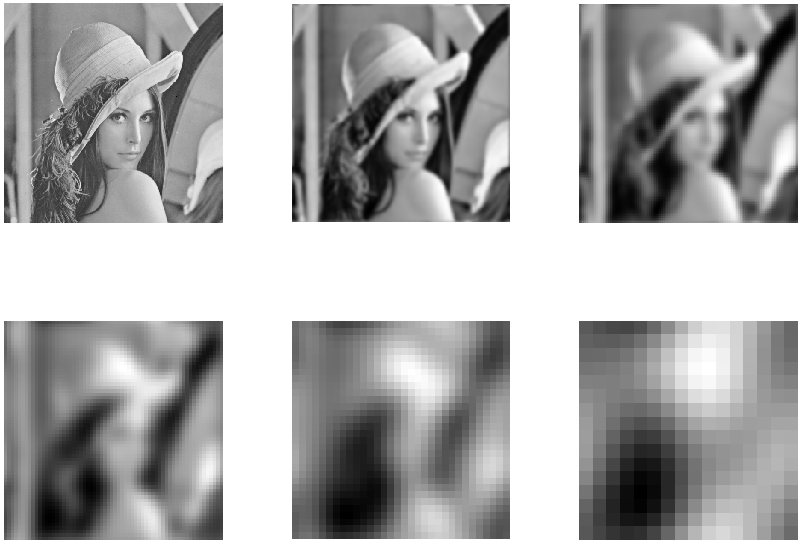
\includegraphics[angle=0,width=\textwidth]{images/gauss_pyr_6_4}
    \caption{6-level Gaussian pyramid with $\sigma = 4$. The
    bottom level of the pyramid is the original image. Note that the
    images have been scaled up to shown the detail of the blurring. The
    images does in fact have different dimensions.}
    \label{gauss_pyramid}
\end{figure}

Moving on to the construction of the Laplacian pyramid, we use the
definition from \citep[Eq. (5.10)]{jahne-digital}:
\begin{equation}
    \mathbi{L}^{p} = \mathbi{G}^{(p)} - \uparrow_2\mathbi{G}^{(p + 1)}, ~~~
    \mathbi{L}^{(P)} = \mathbi{G}^{(P)}
    \label{laplace_pyr_def}
\end{equation}
We need a method for upsampling and such a method is already given in
listing \ref{sample_matlab} where the frequency representation is padded
with zeroes. The method for constructing the Laplacian pyramid is shown
in listing \ref{laplace_pyr_matlab} and an example of a Laplacian
pyramid is shown in Fig. \ref{laplace_pyramid}.

\begin{lstlisting}[caption={Construction of the Laplacian pyramid.
    $P$ is the number of levels in the pyramid. First, the Gaussian
    pyramid is contructed from which we build the Laplacian pyramid
    using Eq. \eqref{laplace_pyr_def}.}, captionpos=b,
    label={laplace_pyr_matlab}, float=b, numbers=none]
    function LP = LaplacianPyramid(I, P, sigma)
        % Generate the Laplacian pyramid to a certain level
        GP = GaussianPyramid(I, P, sigma);
        
        LP = cell(P, 1);
        
        for p = 1:P - 1
            LP{p, 1} = GP{p, 1} - Upsample(GP{p + 1, 1});
        end
        
        LP{P, 1} = GP{P, 1};
    end
\end{lstlisting}

\begin{figure}[!h]
    \centering
    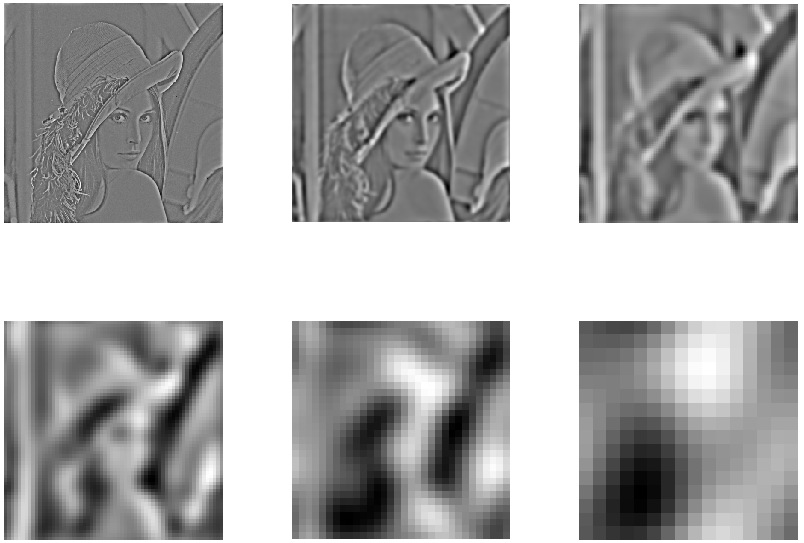
\includegraphics[angle=0,width=\textwidth]{images/laplace_pyr_6_4}
    \caption{6-level Laplacian pyramid built from a Gaussian pyramid
    with $\sigma = 4$. The top level of the pyramid is the same as the
    top of the Gaussian pyramid (see \textbf{fig. \ref{gauss_pyramid}}).
    Again, these images have been scaled up for visual inspection.}
    \label{laplace_pyramid}
\end{figure}

Now we can construct the Laplacian pyramid and from this we can
reconstruct the Gaussian pyramid from which it was built. From
\citep[Eq. (5.11)]{jahne-digital} we have
\begin{equation}
    \mathbi{G}^{(P)} = \mathbi{L}^{(P)}, ~~~ \mathbi{G}^{(p - 1)} =
    \mathbi{L}^{(p - 1)} + \uparrow_2\mathbi{G}^{(p)}
    \label{gauss_reconstruct}
\end{equation}
thus we reconstruct the Gaussian pyramid from top to
bottom\footnote{When constructing the original pyramids this is done
from bottom to top.} as the top the pyramids are the same. Listing
\ref{recon_pyr_matlab} shows the implementation in MATLAB.
Reconstructing the Gaussian pyramid is interesting because the bottom
level of that pyramid is the original image.

\begin{lstlisting}[caption={Reconstruction of the Gaussian pyramid given
    a Laplacian pyramid.}, captionpos=b,
    label={recon_pyr_matlab}, float=b, numbers=none]
    function GP = ReconstructFromLaplacian(LP)
        % Reconstruct the original image from a Laplacian pyramid
        % We do this by reconstructing the Gaussian Pyramid
        P = size(LP,1);
        GP = cell(P, 1);
        
        % The top of the pyramids is equal
        GP{P, 1} = LP{P, 1};
        
        for p = P:-1:2
            GP{p - 1, 1} = LP{p - 1, 1} + Upsample(GP{p, 1});
        end
    end
\end{lstlisting}

Using this scheme I am able to reconstruct the original image entirely
(see fig. \ref{comparison}).  This changes if I were to use a different
method for up- and downsampling the image, i.e. scaling in the spatial
domain using MATLAB's built-in \texttt{imresize()}.

\begin{figure}[!h]
    \centering
    \subfloat[Original]{\label{org_1}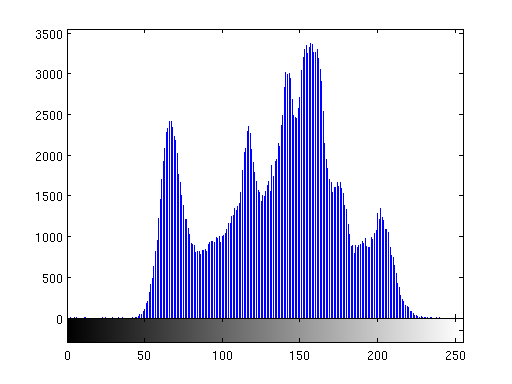
\includegraphics[angle=0,width=0.45\textwidth]{images/org_hist}}\hspace{1em}
    \subfloat[Reconstruction]{\label{ft_1}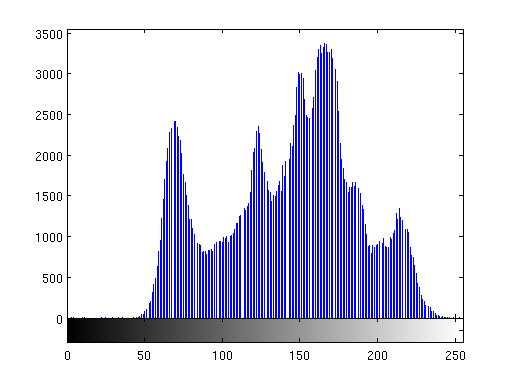
\includegraphics[angle=0,width=0.45\textwidth]{images/recon_hist_1}}\\
    \caption{Histograms of the original and reconstructed image.
    The reconstructed image do not diverge much from the original.
    Actual images are shown in \textbf{fig. \ref{reconstructions}}.}
    \label{comparison}
\end{figure}

\subsubsection*{2. Alternative scheme}
\citep[exercise 5.3]{jahne-digital} presents a different scheme for
constructing the Laplacian pyramid using Laplacians of Gaussians. We can
then construct the Laplacian pyramid in the following manner:
\begin{equation}
    \mathbi{L}^{(p)} = \mathbi{G}^{(p)} - \mathbi{BG}^{(p)}, ~~~
    \mathbi{G}^{(p + 1)} = \downarrow_2 \mathbi{BG}^{(p)}, ~~~
    \mathbi{L}^{(P)} = \mathbi{G}^{(P)}
    \label{alt_laplace}
\end{equation}
Now we want to reconstruct the Gaussian pyramid in a top-down fashion
similar to that in eq. \eqref{gauss_reconstruct} by finding
$\mathbi{G}^{(p - 1)}$. We set $p = p - 1$ in the middle expression from eq.
\eqref{alt_laplace} and get
\begin{align}
    \mathbi{L}^{(p - 1)} & = \mathbi{G}^{(p - 1)} - \mathbi{BG}^{(p - 1)}\\
    \mathbi{G}^{(p - 1)} &= \mathbi{L}^{(p - 1)} + \mathbi{BG}^{(p - 1)}
\end{align}
Yet, this is not enough as we do not know $\mathbi{G}^{(p - 1)}$ in the
second expression on the right side. By inspecting the structure of the
Gaussian pyramid we see that we can find $\mathbi{G}^{(p - 1)}$ by
upsampling $\mathbi{G}^{(p)}$ and applying the inverse convolution, i.e.
\begin{equation}
    \mathbi{G}^{(p - 1)} = \mathbi{B}^{-1}\uparrow_2\mathbi{G}^{(p)}
\end{equation}

We have to find the inverse convolution. Convolution equals
multiplication in the frequency domain, thus deconvolution is division.
Originally we have convoluted with a Gaussian which have tails that
converge zero. This means that in the deconvolution we have to divide by
zero or guess what the correct value for a ``zeroed out'' pixel
originally was. This is very hard and this method is therefore
abandoned.

Alternatively, we can insert the expression for $\mathbi{G}^{(p - 1)}$
and we end with Eq. (5.11) from \citep{jahne-digital} again. This is not
quite right, as we cannot find the exact deconvolution.

\begin{align}
    \mathbi{B}^{-1}\uparrow_2\mathbi{G}^{(p)} & = \mathbi{L}^{(p - 1)} + \mathbi{BB}^{-1}\uparrow_2\mathbi{G}^{(p)}\\
    \mathbi{G}^{(p - 1)} & = \mathbi{L}^{(p - 1)} + \uparrow_2\mathbi{G}^{(p)}\\
\end{align}

\subsubsection*{3. Implementing alternative scheme}

I have implemented the alternative construction of the Laplacian pyramid
and the code can be found in listing \ref{alt_laplace_matlab}. This code
is equal to the second part of the question. The pyramid that is
produced is shown in fig. \ref{alt_laplace_pyramid}.

Using the same reconstruction as before the original image is restored
from the Laplacian pyramid. Visually one cannot see the difference, but
inspecting the histogram shows some difference (see fig.
\ref{alt_comparison}). The original and the reconstructed images are
shown in fig. \ref{reconstructions}.

\begin{lstlisting}[caption={Alternative construction of the Laplacian
    pyramid using difference of two gaussians at different scales.}, captionpos=b,
    label={alt_laplace_matlab}, float=b, numbers=none]
    function LP = AlternativeLaplacianPyramid(I, P, sigma)
       % Construct the Laplacian pyramid differently
       GP = GaussianPyramid(I, P, sigma);
       LP = cell(P, 1);

       for p = 1:P - 1
           LP{p, 1} = GP{p, 1} - Gauss(GP{p, 1}, sigma);
       end
       
       LP{P, 1} = GP{P, 1};
    end
\end{lstlisting}

\begin{figure}[!h]
    \centering
    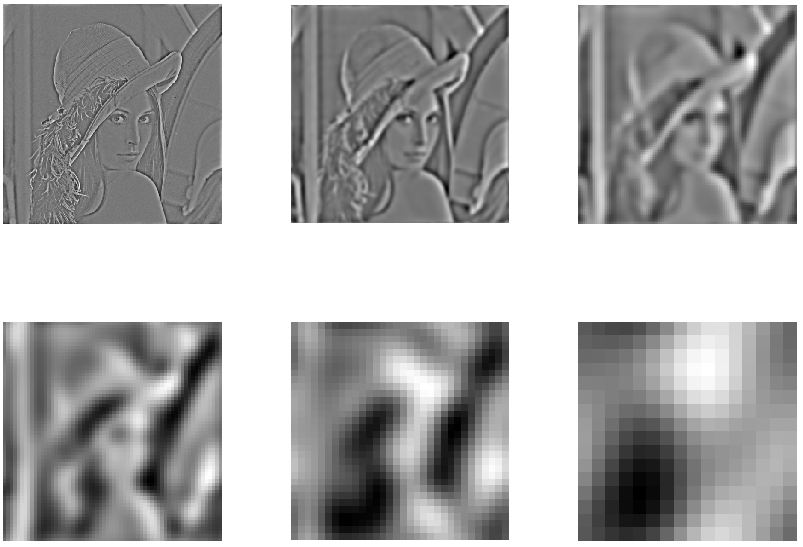
\includegraphics[angle=0,width=\textwidth]{images/alt_laplace_pyr_6_4}
    \caption{The alternative 6-level Laplacian pyramid with $\sigma =
    4$. Visually this is identical to the one shown in \textbf{fig.
    \ref{laplace_pyramid}} but they do in fact have minor differences.}
    \label{alt_laplace_pyramid}
\end{figure}

\begin{figure}[!h]
    \centering
    \subfloat[Original]{\label{org_hist2}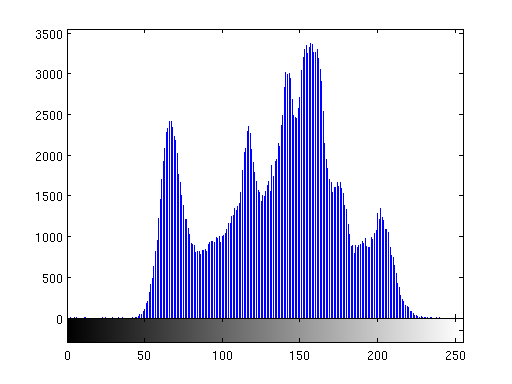
\includegraphics[angle=0,width=0.45\textwidth]{images/org_hist}}\hspace{1em}
    \subfloat[Reconstruction (alternative)]{\label{alt_hist}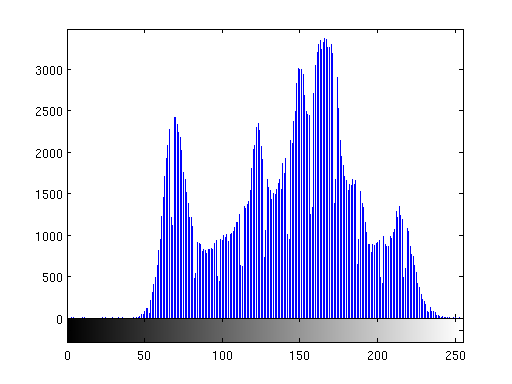
\includegraphics[angle=0,width=0.45\textwidth]{images/recon_hist_2}}\\
    \caption{Comparison of histograms of the original and the
    reconstruction from the alternative construction of the Laplacian
    pyramid. The reconstruction do have some minor differences. In some
    areas, almost systematic, we see a slight decrease in color concentration.}
    \label{alt_comparison}
\end{figure}

\begin{figure}[!h]
    \centering
    \subfloat[Original]{\label{org}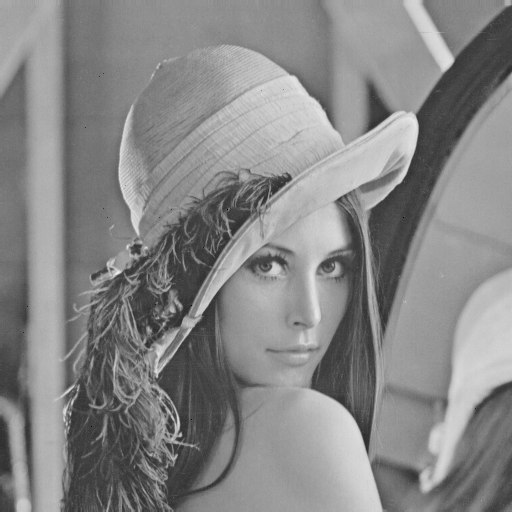
\includegraphics[angle=0,width=0.30\textwidth]{images/org}}\hspace{1em}
    \subfloat[Reconstruction]{\label{reconst1}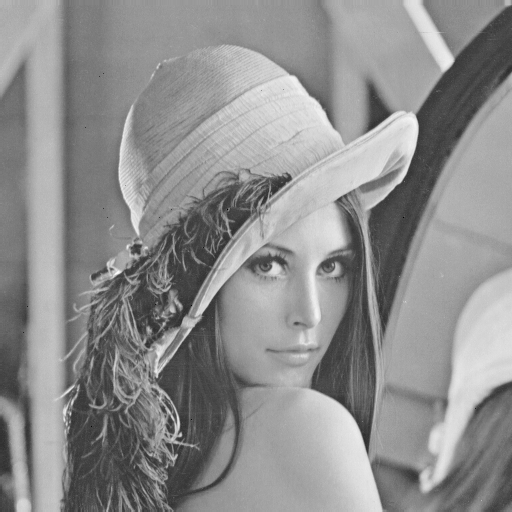
\includegraphics[angle=0,width=0.30\textwidth]{images/reconst1}}\hspace{1em}
    \subfloat[Reconstruction (alternative)]{\label{reconst2}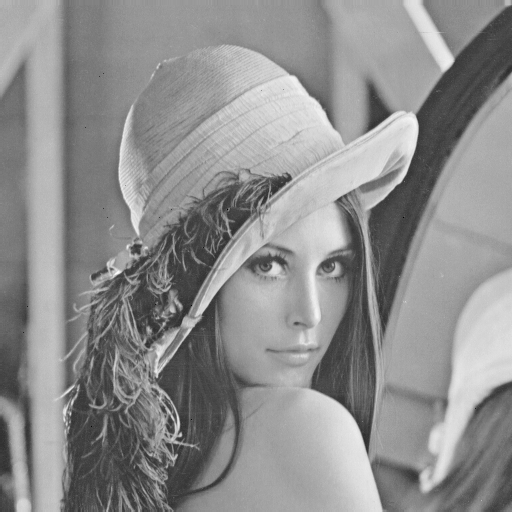
\includegraphics[angle=0,width=0.30\textwidth]{images/reconst2}}
    \caption{Comparison of reconstructed images. Both reconstructions
    are made from a Laplacian pyramid with 6 levels and $\sigma = 4$. No
    visble artifacts have been observed using different values for the
    number of levels or $\sigma$.}
    \label{reconstructions}
\end{figure}

\subsubsection*{Final remarks}
Just for clarification to the actual given assignment I will sum up my
results with respect to the different parts.

For \emph{part 1} I have implemented Eqs. (5.8), (5.10) and (5.11) from
\citep{jahne-digital}.

For \emph{part 2} we see that the alternative construction of the
Laplacian pyramid actually \emph{is} the subtraction of two Gaussians
at different scales, i.e. this is just the same as the equation given in
\citep[exercise 5.3]{jahne-digital}. I have implemented this and
reconstructed using the previous method for reconstruction.

\subsection*{Question 4.2}

%%%%%%%%%%%%%%%%%%%%%%%%%%%%%%%%%%%%%%%%%%%%%%%%%%%%%%%%%%%%%%%%%%%%
% Formal stuff

\bibliographystyle{abbrvnat}
\bibliography{bibliography}
%\addcontentsline{toc}{chapter}{Litteratur}

\end{document}

% vim: set tw=72 spell spelllang=en:
